\documentclass[margins=1mm]{standalone}

\usepackage{tikz}
\usetikzlibrary{calc,shapes.arrows,arrows,arrows.meta,shapes,decorations,positioning,}

\begin{document}
	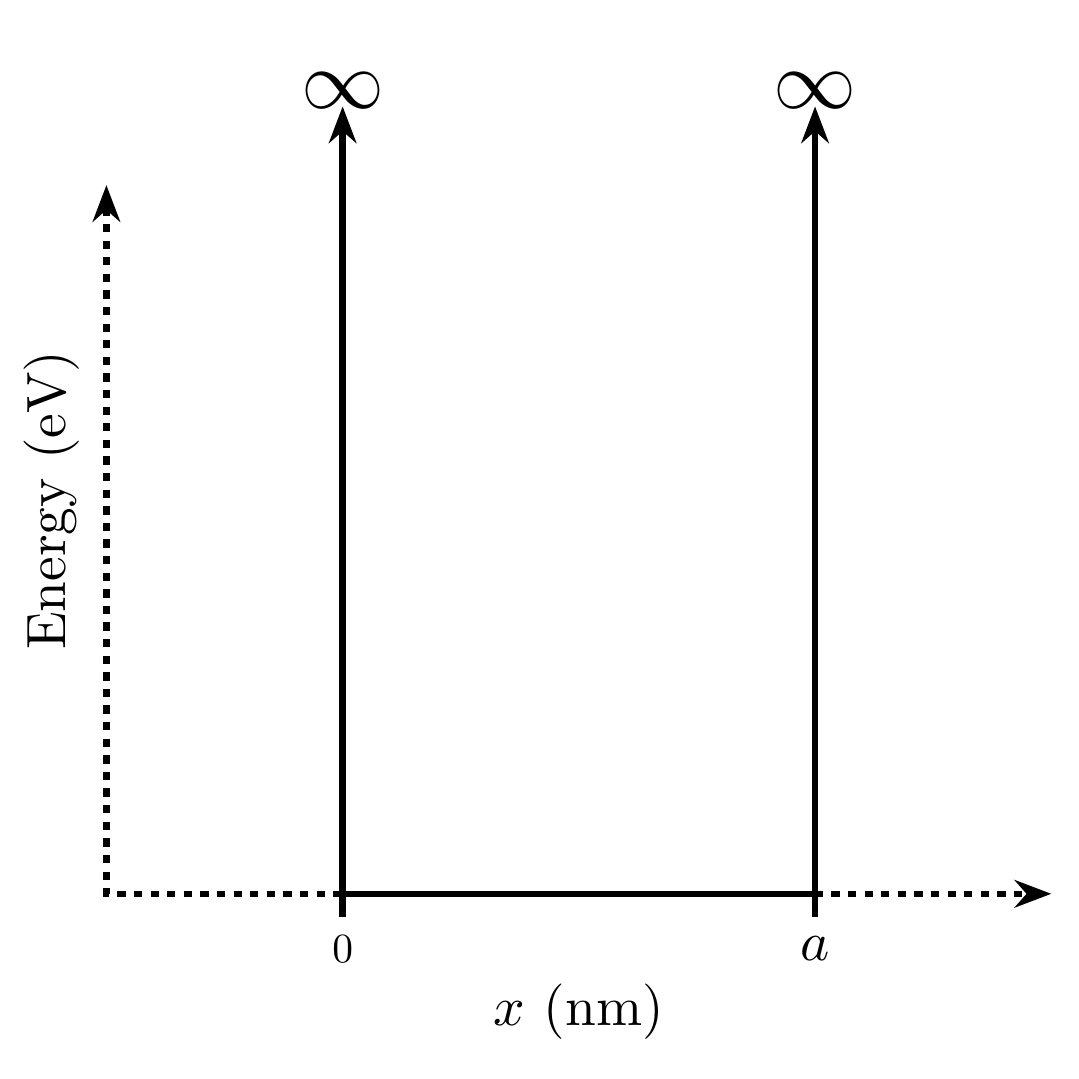
\begin{tikzpicture}
		\useasboundingbox (-7,-2) rectangle (6,11);
		\draw[{Stealth[scale=1]}-{Stealth[scale=1]},line width=0.8mm](-3,10)--(-3,0)--(3,0)--(3,10);
		\node[scale=3] at (-3,10.2) {$\infty$};
		\node[scale=3] at (3,10.2) {$\infty$};
		\draw[{Stealth[scale=1]}-{Stealth[scale=1]},line width=0.8mm,dashed] (-6,9)--(-6,0)--(6,0);
		\draw[line width=0.8mm] (-3,0)--(-3,-0.3);
		\node[scale=1.5] at (-3,-0.7){0};
		\draw[line width=0.8mm] (3,0)--(3,-0.3);
		\node[scale=2] at (3,-0.7){$a$};
		\node[scale=2] at (0,-1.5) {$x$ (nm)};
		\node[scale=2, rotate=90] at (-6.7,5){Energy (eV)};
		
	\end{tikzpicture}
	
	
	
\end{document}